\documentclass[xcolor={dvipsnames},pdf, hyperref={colorlinks=true, citecolor=ForestGreen, linkcolor=BlueViolet, urlcolor=Magenta}]{beamer}
\usetheme{Frankfurt}  
\usecolortheme{whale}
\usepackage{tikz} 
\usepackage{graphicx}
\usepackage{dsfont}
\usepackage{hyperref}
\usepackage{alltt}
\usepackage{enumerate}
\usepackage{amsthm}
\theoremstyle{definition}
\newtheorem{exmp}{Example}[section]
\usepackage{verbatim}               % useful for \begin{comment} and \end{comment}
\usepackage{eurosym}                % used for euro symbol
\usepackage{caption} 
\usepackage{graphicx}
\usepackage{adjustbox}
\graphicspath{{Figures/}}
\usepackage{subcaption}
\usepackage{color}
\usepackage{float}
\usepackage{amssymb}
\usepackage{sgamevar}
\usepackage{remreset}% tiny package containing just the \@removefromreset command
\makeatletter
\@removefromreset{subsection}{section}
\makeatother
\setcounter{subsection}{1}



\newcommand{\defn}[1]{\textbf{#1}}


%Instructor version
\newcommand{\blank}[0]{}
\newcommand{\ddp}[1]{{\textcolor{ForestGreen}{#1}}} 
\newcommand{\dd}[1]{{\underline{\textcolor{ForestGreen}{#1}}}}

%Student version
%\newcommand{\blank}[0]{\vspace{2em}}
%\newcommand{\dd}[1]{\underline{\hspace{3cm}}} 
%\newcommand{\ddp}[1]{}

\addtobeamertemplate{navigation symbols}{}{%
	\usebeamerfont{footline}%
	\usebeamercolor[fg]{footline}%
	\hspace{1em}%
	\insertframenumber/\inserttotalframenumber
}

\section{Introduction}

%% preamble
\title{Savings and Investment}
\author{David A. D\'iaz}
\institute{UNC Chapel Hill}
\date{}

\AtBeginSection[] %Section links on slides

\begin{document} 
	
	\begin{frame}
		
		\titlepage
		
	\end{frame}


\begin{frame}{Savings and Investment in the U.S.}
\begin{itemize}
	\item This section looks at how \textbf{financial institutions} match one person's savings to another person's investment. 
	\item \defn{Financial markets:} Financial institutions through which savers can \underline{directly} provide funds to borrowers.

\end{itemize}
\end{frame}

\begin{frame}{Savings and Investment in the U.S.}

	\begin{enumerate}
		\item The bond market
		\begin{itemize}
			\item Bond - A certificate of indebtedness.
			\item Corporations, governments, etc. issue (sell) bonds in order to finance purchases. 
			\item Important: Buyer of the bond is the lender, seller is the borrower.
			\item Interest rate on the bond varies with the level of risk (e.g., time to maturity, credit risk)
		\end{itemize}  

		
	\end{enumerate}

\end{frame}


\begin{frame}{Savings and Investment in the U.S.}

\begin{enumerate}
\setcounter{enumi}{1}
	\item The stock market
	\begin{itemize}
		\item Stock - A claim to partial ownership in a firm.
		\item  Firms sell stock to raise money (equity finance).
		\item Compared to bonds, stocks offer higher returns but are also riskier.
	\end{itemize}  
	
\end{enumerate}

\end{frame}



\begin{frame}{Savings and Investment in the U.S.}
\begin{itemize}
	\item \defn{Financial intermediaries:} Financial institutions through with savers can \underline{indirectly} provide funds to borrowers.
	
	\begin{enumerate}
		\item Banks: Take deposits from people who want to save and use deposits to make loans to people who wish to borrow.
		\item Mutual funds: Institutions that sell shares to the public and use the proceeds to buy a portfolio of stocks and bonds. Allow people with small amounts of money to diversify.
	\end{enumerate}
\end{itemize}
\end{frame}

\section{National Income}

\begin{frame}{The National Income Accounts}
\begin{itemize}
	\item Recall that GDP can be written as the sum of the four components of expenditure: 
	\begin{equation*}
	Y = C + I + G + NX
	\end{equation*}
	
	\item For the purposes of this section, we will assume that the economy is \dd{closed}. This is an economy that does not not engage in \dd{international trade} or in international borrowing and lending. Thus, \dd{$NX = 0$}.
	\item Then, we can write 
	
	\[\ddp{Y = C + I + G \Rightarrow I = Y - C - G}\]
\end{itemize}
\end{frame}

\begin{frame}{The National Income Accounts}
\begin{itemize}
	\item The term \dd{$Y - C - G$} represents the total income in the economy that remains after paying for consumption and government purchases. We call this amount \dd{national savings}. 
	\item Replacing this term with $S$, we have that \dd{savings} equals \dd{investment}.
\end{itemize}
\end{frame}

\begin{frame}{The National Income Accounts}
\begin{itemize}
	\item Let $T$ denote the amount the government collects from households in \dd{taxes} minus the amount it pays back in the form of \dd{transfer payments}.
	\item Given this, we can write national saving as \ddp{\[S = Y - C - G = (Y - C - T) + (T - G)\]}
\end{itemize}
\end{frame}

\begin{frame}{The National Income Accounts}
\begin{itemize}
	\item \defn{Private saving:} The amount of income households have left after paying their taxes and for consumption: \dd{$Y - C - T$}
	\item \defn{Public saving:} The tax revenue that the government has after paying for its spending: \dd{$T - G$}
	
	\item Two cases of note for public saving:
	\begin{enumerate}
		\item $T > G$: Budget surplus - government is receiving more than it spends.
		\item $T < G$: Budget deficit - government is spending more than it receives.
	\end{enumerate}
\end{itemize}
\end{frame}

\begin{frame}{The National Income Accounts}
\begin{exmp}
	Suppose GDP is \$8 trillion, taxes are \$1.5 trillion, private saving is \$.5 trillion, and public saving is \$.2 trillion. Assuming a closed economy, what is consumption, government purchases, national saving, and investment?
\end{exmp} 
\ddp{$Y = 8$, $T = 1.5$ \\
	\pause Private saving = $Y - T - C = .5 \Rightarrow 8 - 1.5 - C = .5 \Rightarrow C = 6T$. 
	\\
	\pause Public saving = $T - G = .2T \Rightarrow 1.5 - G = .2 \Rightarrow G = 1.3T$. 
	\\
	\pause National saving = private + public saving = national investment = $.5T + .2T = .7T$.}
\end{frame}

\begin{frame}{Savings versus Investment}
\begin{itemize}
		\item Savings: Occurs when income exceeds consumption
		\item Investment: Refers to the purchase of new capital
	\end{itemize}
\end{frame}

\begin{frame}{Savings versus Investment}

\begin{exmp} For each of the following, state whether the transaction would be considered savings or investment as defined by a macroeconomist.
	\begin{enumerate}
		\item Your family takes out a mortgage and purchases a new home.
		\item You use \$200 of your \$800 paycheck to purchase stock in Apple.
		\item You borrow \$2,000 from a bank in order to purchase a van for your new ghost hunting business. 
	\end{enumerate}
\end{exmp}

\ddp{\pause Investment (remember home purchases are included in $I$) \\
\pause Savings \\
Investment}
\end{frame}

\section{The Loanable Funds Market}

\begin{frame}{The Loanable Funds Market}
\begin{itemize}
	\item \defn{The market for loanable funds:} The market in which those who want to save supply funds and those who want to borrow to invest demand funds.
	\item Assumptions:
	\begin{itemize}
		\item This is the only financial market.
		\item There is one interest rate, which is both the return to \dd{saving} and the cost of \dd{borrowing}.
	\end{itemize}
\end{itemize}
\end{frame}

\begin{frame}{The Loanable Funds Market}
\begin{itemize}

		\item Supply: Determined by savers - households who have extra income to save and lend out (either directly or indirectly)
		\item Demand: Determined by borrowers - households and firms who wish to borrow in order to make investments
	
\item The price of a loan is the \dd{real interest rate}. It represents the amount that \dd{borrowers} pay for loans and the amount \dd{savers} receive on their savings.
	
\end{itemize}
\end{frame}

\begin{frame}{The Loanable Funds Market}
\begin{itemize}
	\item A higher interest rate means that the cost of borrowing is \dd{greater}, so as the interest rate increases, the quantity of loanable funds demanded will \dd{decrease}. 
	\item Thus, the demand curve for loanable funds is \dd{downward-sloping}. 
\end{itemize}
\end{frame}

\begin{frame}{The Loanable Funds Market}
\begin{itemize}
	\item Conversely, a higher interest rate means that the returns to savings is \dd{greater}, so as the interest rate increases, the quantity of loanable funds supplied will \dd{increase}. 
	\item Thus, the supply curve for loanable funds is \dd{upward-sloping}.
\end{itemize}
\end{frame}

\begin{frame}[b]{The Loanable Funds Market}
	\begin{figure}[H]
	\centering
	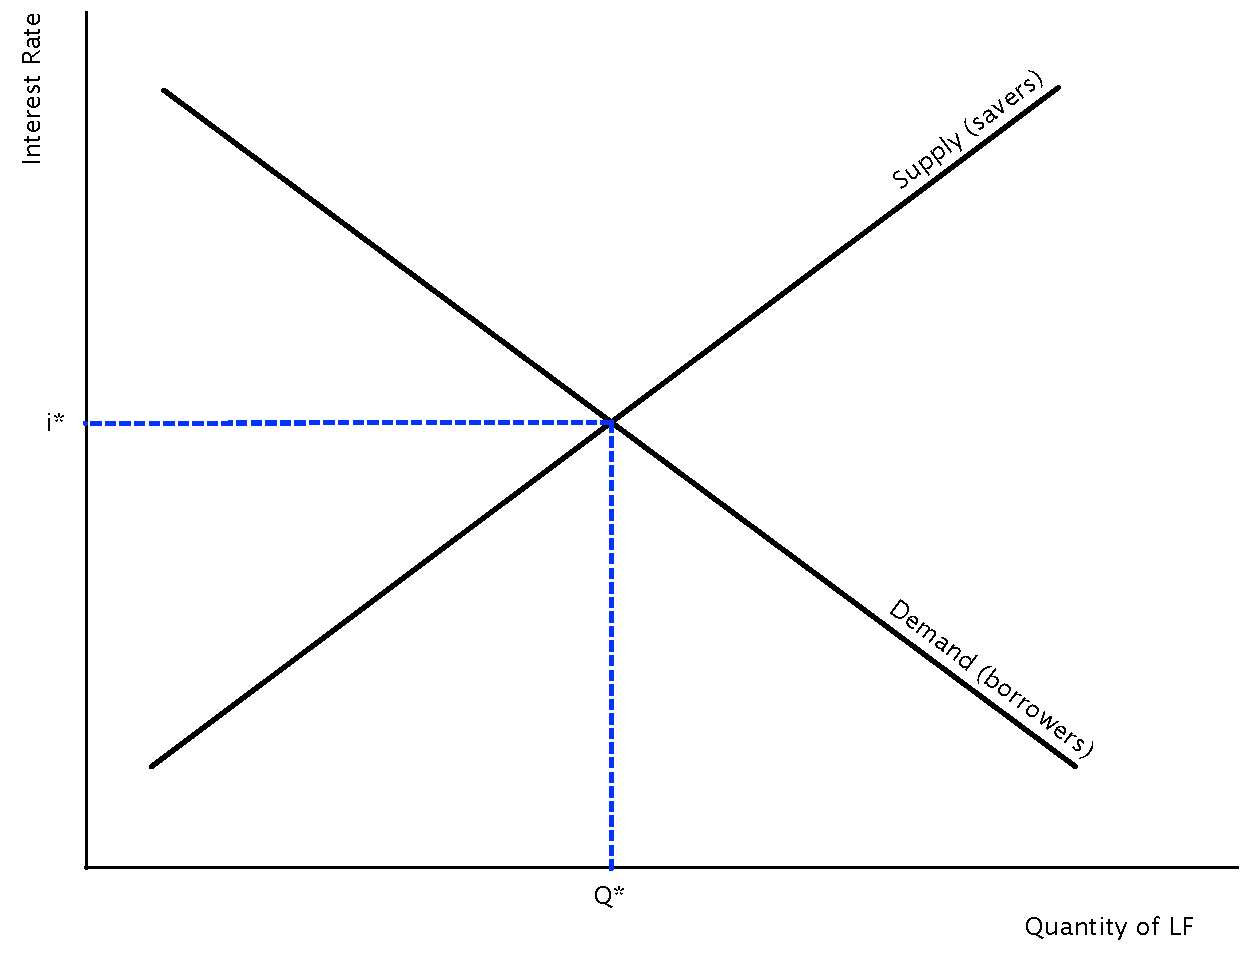
\includegraphics[scale=.40]{plot89.pdf}
	\caption{The Market for Loanable Funds}
\end{figure}
\end{frame}

\begin{frame}{The Loanable Funds Market}
\begin{itemize}
	\item The analysis of the loanable funds market is the same as what we saw in other markets. 
	\item If the interest rate is too high, then there will be a \dd{surplus} of loanable funds because the quantity demanded will be \dd{less} than the quantity supplied. 
	\item As such, there will be \dd{downward} pressure on the interest rate until it reaches the equilibrium rate. 
	\item If the interest rate is too low, then there will be a \dd{shortage} of loanable funds, and thus \dd{upward} pressure on the interest rate.
\end{itemize}
\end{frame}

\begin{frame}{The Loanable Funds Market}
\begin{itemize}
	\item Importantly, because the \dd{real} interest rate more accurately reflects the actual return to savings and cost of borrowing, the equilibrium in the loanable funds market is interpreted as determining the \textit{real} interest rate in the economy.
	\item Several policies can affect the market for loanable funds by encouraging more savings or investment. 
\end{itemize}
\end{frame}

\begin{frame}[b]{The Loanable Funds Market}
	\begin{figure}[H]
	\centering
	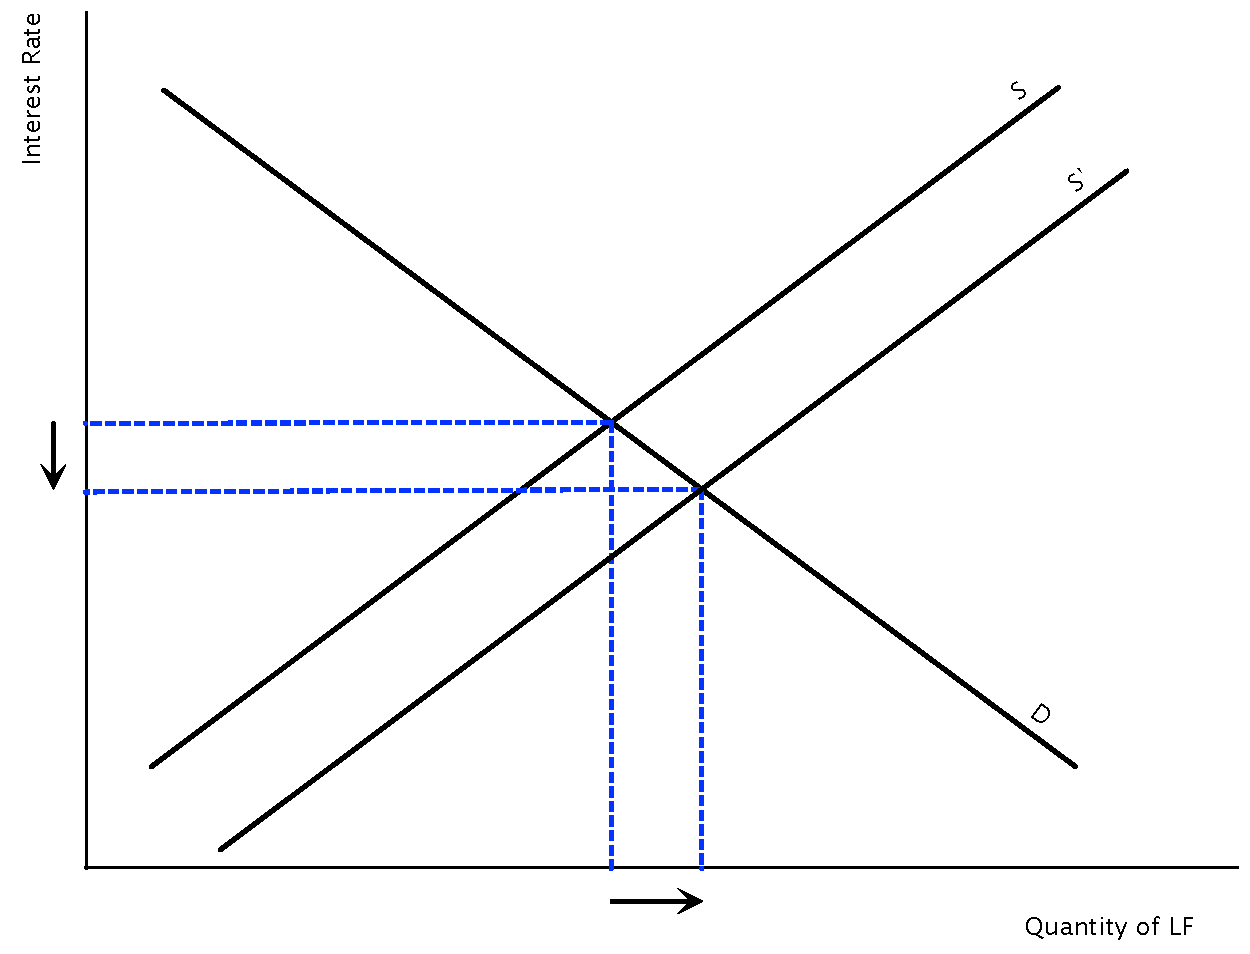
\includegraphics[scale=.40]{plot90.pdf}
	\caption{Saving Incentives}
\end{figure}
\end{frame}

\begin{frame}[b]{The Loanable Funds Market}
	\begin{figure}[H]
		\centering
		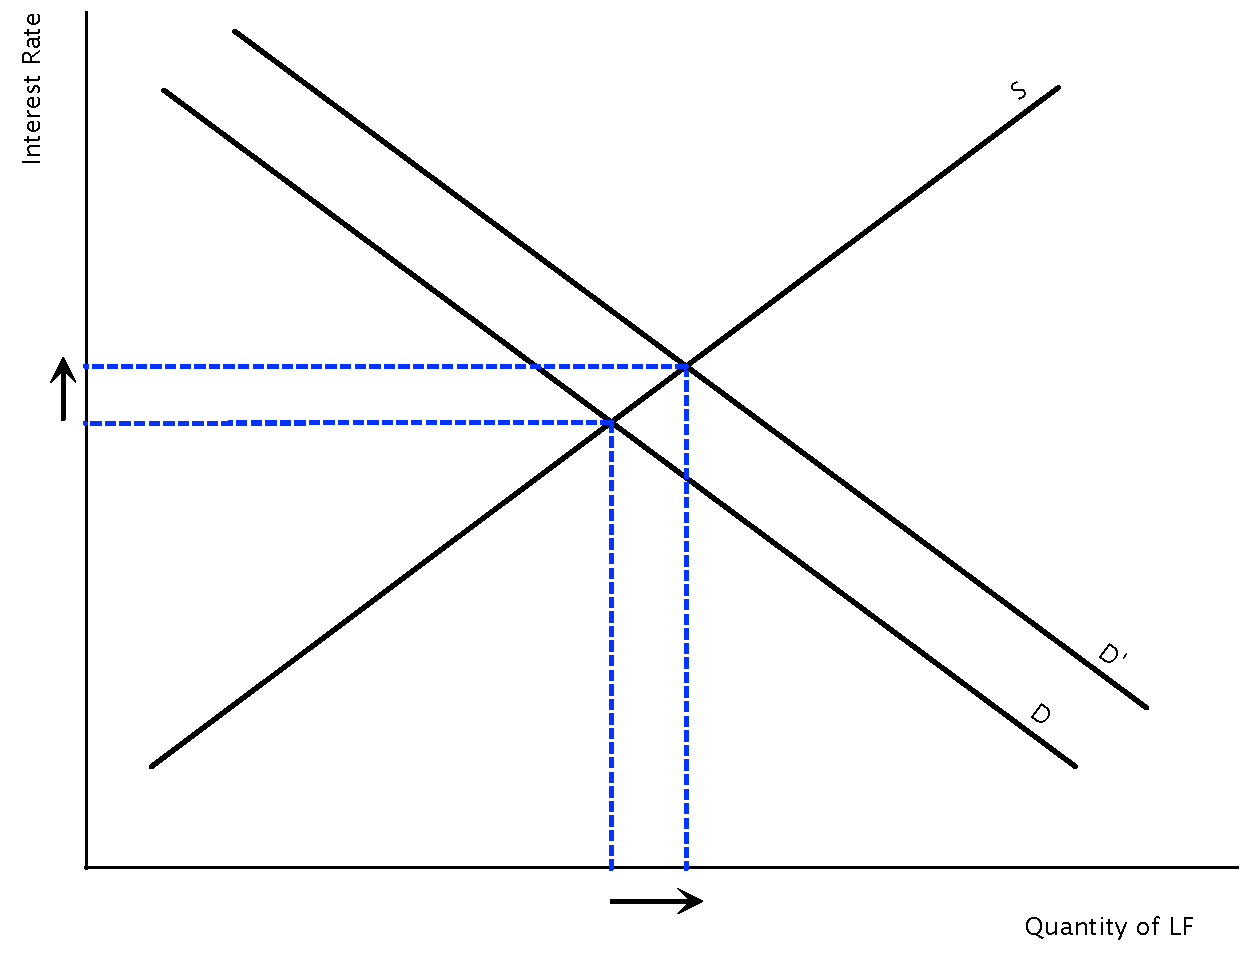
\includegraphics[scale=.40]{plot91.pdf}
		\caption{Investment Incentives}
	\end{figure}
\end{frame}

\begin{frame}{The Loanable Funds Market}
\begin{itemize}
	\item 	\defn{Crowding out:} A decrease in investment and consumption that results from government borrowing. A deficit decreases investment because it causes the equilibrium interest rate to increase.
\end{itemize}
	\begin{figure}[H]
		\centering
	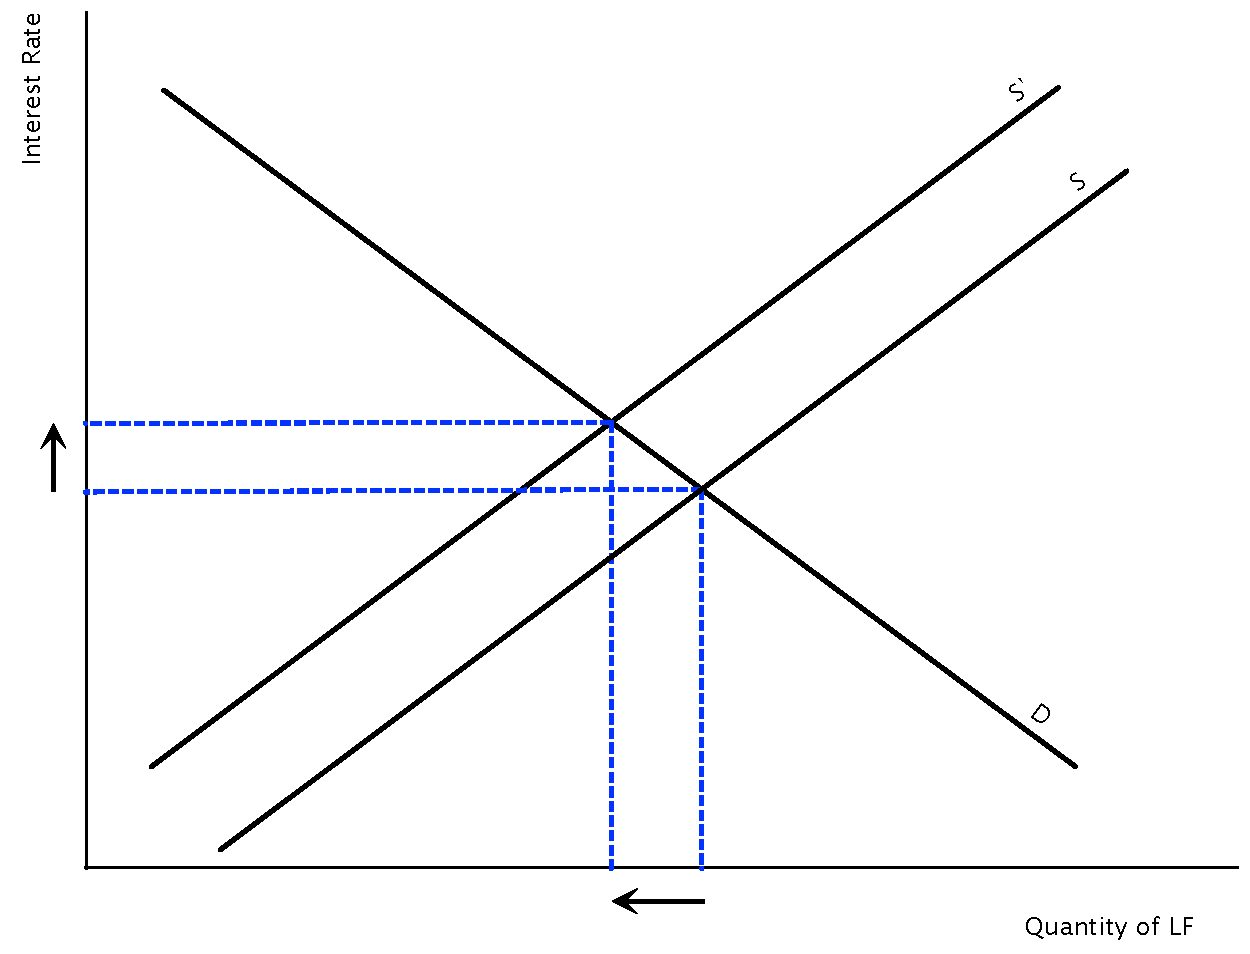
\includegraphics[scale=.35]{plot92.pdf}
	\caption{Government Deficits}
	\end{figure}
\end{frame}

\begin{frame}{The Loanable Funds Market}
\begin{exmp}
	Use the market for loanable funds to explain what will happen to the quantity of savings, quantity of investment, and the interest rate when each of the following occur.
	\begin{enumerate}[(a)]
		\item A technological advance increases the profitability of new investment to firms.
		\item The federal budget deficit increases.
		\item A consumption tax is imposed.
	\end{enumerate}
\end{exmp}
\end{frame}

\section{The Time Value of Money}

\begin{frame}{The Time Value of Money}
\begin{itemize}
	\item \defn{Present value:} The amount of money today that would be needed to produce a future amount using prevailing interest rates.
	
	\item \defn{Future value:} The amount of money in the future that a certain amount of money today will yield given prevailing interest rates.
	
	\item Formula: 
	\[PV = \frac{FV}{(1+i)^t}\] 
	where $t$ represents the number of periods to discount.
	
	\item Note that as the interest rate increases, the present value \dd{decreases}.
\end{itemize}
\end{frame}

\begin{frame}{The Time Value of Money}
\begin{exmp} If the interest rate is 10\%, then what is the present value of \$100 to be paid in two years? What if the interest rate was 15\%?
\end{exmp}

\ddp{\pause PV = 100/(1.10)$^2$ = 82.64 \\
	\pause PV = 100/(1.15)$^2$ = 75.61}

\end{frame}

\begin{frame}{The Time Value of Money}
\begin{exmp} 
	The price of a bond is the sum of the present value of its future payments. Suppose you purchase a bond today that promises to pay \$75 one year from now, \$75 two years from now, and \$1075 three years from now. If the interest rate is 7.5\%, what is the price of this bond today? 
\end{exmp}
\ddp{\pause P = 75/1.075 + 75/1.075$^2$ + 1075/1.075$^3$ = 1000.}
\end{frame}

\begin{frame}{The Time Value of Money}
\begin{exmp}
	A year after you buy your bond, you decide to sell it in order purchase a new computer. If the market interest rate is still 7.5\%, what is the fair price for your bond? What if the interest rate was 10\%?
\end{exmp}
\ddp{\pause P = 75/1.075 + 1075/1.075$^2$ = 1000 \\
\pause 	P = 75/1.10 + 1075/1.10$^2$ = 956.61.\\}
\begin{itemize}
	\item Note that the price of a bond and interest rates are \dd{inversely} related.
\end{itemize}
\end{frame}

\begin{frame}{Readings and Assignments}
\begin{itemize}
	\item Today: Mankiw Ch. 26
	\item Next time: Mankiw Ch. 28
	\item Problem Set 5, section 3
\end{itemize}
\end{frame}

\end{document}